\section{تعريف النظام ومكوناته الأساسية}
\label{sec:components}

تُعرّف أنظمة التحكم بالحركة (\textenglish{Motion Control Systems}) بأنها أنظمة هندسية متكاملة تُعنى بالتحكم الدقيق والمستمر في المتغيرات الديناميكية للحركة، والتي تشمل الموضع (\textenglish{Position})، السرعة (\textenglish{Velocity})، والتسارع (\textenglish{Acceleration}). تلعب هذه الأنظمة دوراً محورياً في تطبيقات الأتمتة الصناعية الحديثة، حيث تضمن تنفيذ المناورات الحركية المعقدة بكفاءة وتكرارية عالية وثبات ديناميكي، لا سيما في الآلات ذات التحكم الرقمي (\textenglish{CNC}) والمنظومات الروبوتية المتقدمة.

% المخطط الصندوقي للمكونات
\begin{figure}[h!]
    \centering
    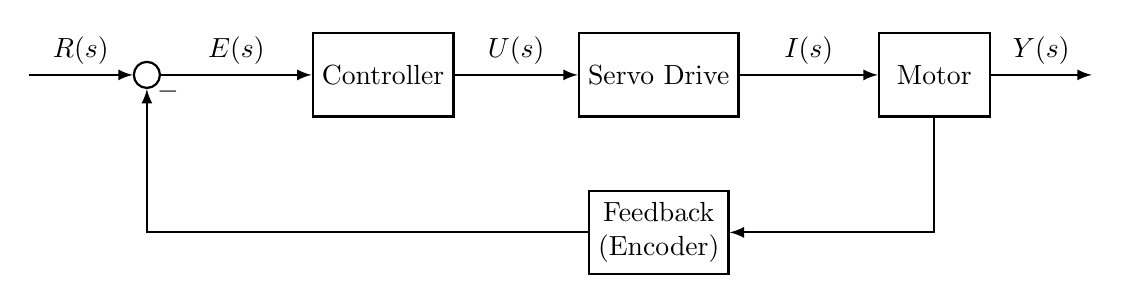
\begin{tikzpicture}[auto, node distance=2.5cm, >=latex]
        % تعريف أشكال الكتل
        \tikzstyle{block} = [draw, rectangle, minimum height=3em, minimum width=4em, align=center, thick]
        \tikzstyle{sum} = [draw, circle, node distance=1.5cm, thick]
        \tikzstyle{input} = [coordinate]
        \tikzstyle{output} = [coordinate]

        % رسم العقد (Nodes)
        \node [input] (ref) {};
        \node [sum, right of=ref] (sum) {};
        \node [block, right of=sum, node distance=3cm] (controller) {\textenglish{Controller}};
        \node [block, right of=controller, node distance=3.5cm] (drive) {\textenglish{Servo Drive}};
        \node [block, right of=drive, node distance=3.5cm] (motor) {\textenglish{Motor}};
        \node [output, right of=motor, node distance=2cm] (out) {};
        \node [block, below of=drive, node distance=2cm] (feedback) {\textenglish{Feedback}\\\textenglish{(Encoder)}};

        % رسم الأسهم والمسارات (Edges)
        \draw [->, thick] (ref) -- node [above] {$R(s)$} (sum);
        \draw [->, thick] (sum) -- node [above] {$E(s)$} (controller);
        \draw [->, thick] (controller) -- node [above] {$U(s)$} (drive);
        \draw [->, thick] (drive) -- node [above] {$I(s)$} (motor);
        \draw [->, thick] (motor) -- node [above] (y) {$Y(s)$} (out);
        \draw [->, thick] (motor) |- (feedback);
        \draw [->, thick] (feedback) -| node[pos=0.99, right] {$-$} (sum);
    \end{tikzpicture}
    \caption{\centering{مخطط صندوقي يوضح المكونات الأساسية لنظام التحكم بالحركة ذو الحلقة المغلقة}}
    \label{fig:motion_components}
\end{figure}

\subsection{مسار الإشارة والمكونات الفعالة}
كما يتبين من المخطط الصندوقي في الشكل (\ref{fig:motion_components})، يتكون نظام التحكم بالحركة الحلقي المغلق من أربعة عناصر أساسية تتفاعل ديناميكياً فيما بينها لضمان تتبع المسار المطلوب بدقة:

\begin{enumerate}
    \item \textbf{وحدة التحكم بالحركة (\textenglish{Motion Controller}):}
    تمثل العقل المدبر ومصدر القرار في النظام. تستقبل هذه الوحدة إشارة الخطأ $E(s)$ الناتجة عن مقارنة الدخل المرجعي $R(s)$ مع التغذية الراجعة. تتلخص وظيفتها في توليد وتخطيط مسار الحركة الزمني (\textenglish{Trajectory Generation})، ومن ثم إنتاج إشارة تحكم $U(s)$ بناءً على خوارزميات التحكم المطبقة (مثل \textenglish{PID}).
    
    \item \textbf{مُشغل القدرة أو المكبر (\textenglish{Servo Drive / Amplifier}):}
    يعمل كوسيط طاقة بين وحدة التحكم والمحرك. يستقبل المشغل إشارة التحكم القيادية $U(s)$، ويقوم بتضخيمها وتحويلها إلى كميات تيار وجهد ملائمة $I(s)$ لتوليد العزم المغناطيسي المطلوب في المحرك، مع مراعاة حماية النظام من التيارات الزائدة.
    
    \item \textbf{المُحرك (\textenglish{Actuator / Servo Motor}):}
    هو العضو التنفيذي المسؤول عن تحويل الطاقة الكهربائية القادمة من المشغل إلى طاقة ميكانيكية حركية $Y(s)$. تمتاز محركات السيرفو بالقدرة على تحمل أحمال متغيرة وتوفير تسارعات عالية بفضل انخفاض عزم القصور الذاتي لعضوها الدوار.
    
    \item \textbf{حساس التغذية الراجعة (\textenglish{Feedback Device}):}
    يمثل عين النظام التي تراقب الأداء في الوقت الحقيقي. يُثبت هذا الحساس (مثل المشفرات \textenglish{Encoders}) لقياس المخرج الفعلي $Y(s)$، وإرسال هذه القياسات عودةً إلى نقطة المقارنة لإغلاق حلقة التحكم وتصحيح أي انحراف عن المسار المستهدف بشكل مستمر.
\end{enumerate}